% !TEX root = ../thesis.tex

\section{Social Signal Prediction in Haggling Scenario}
We use our Haggling scenario as an example problem of social signal prediction to computationally model triadic interaction. In this section, we specifically define the input and output signals used in our modeling, and then present two social signal predicting problems, predicting speaking status and predicting social formation, by describing their problem definitions and implementation details. Note that we focus on estimating the target person's concurrent signals by taking other individuals' signals as input as defined in Equation~\ref{equation:F_ours} to simplify the problem, rather than forecasting the future signals.


\begin{figure}[t]
	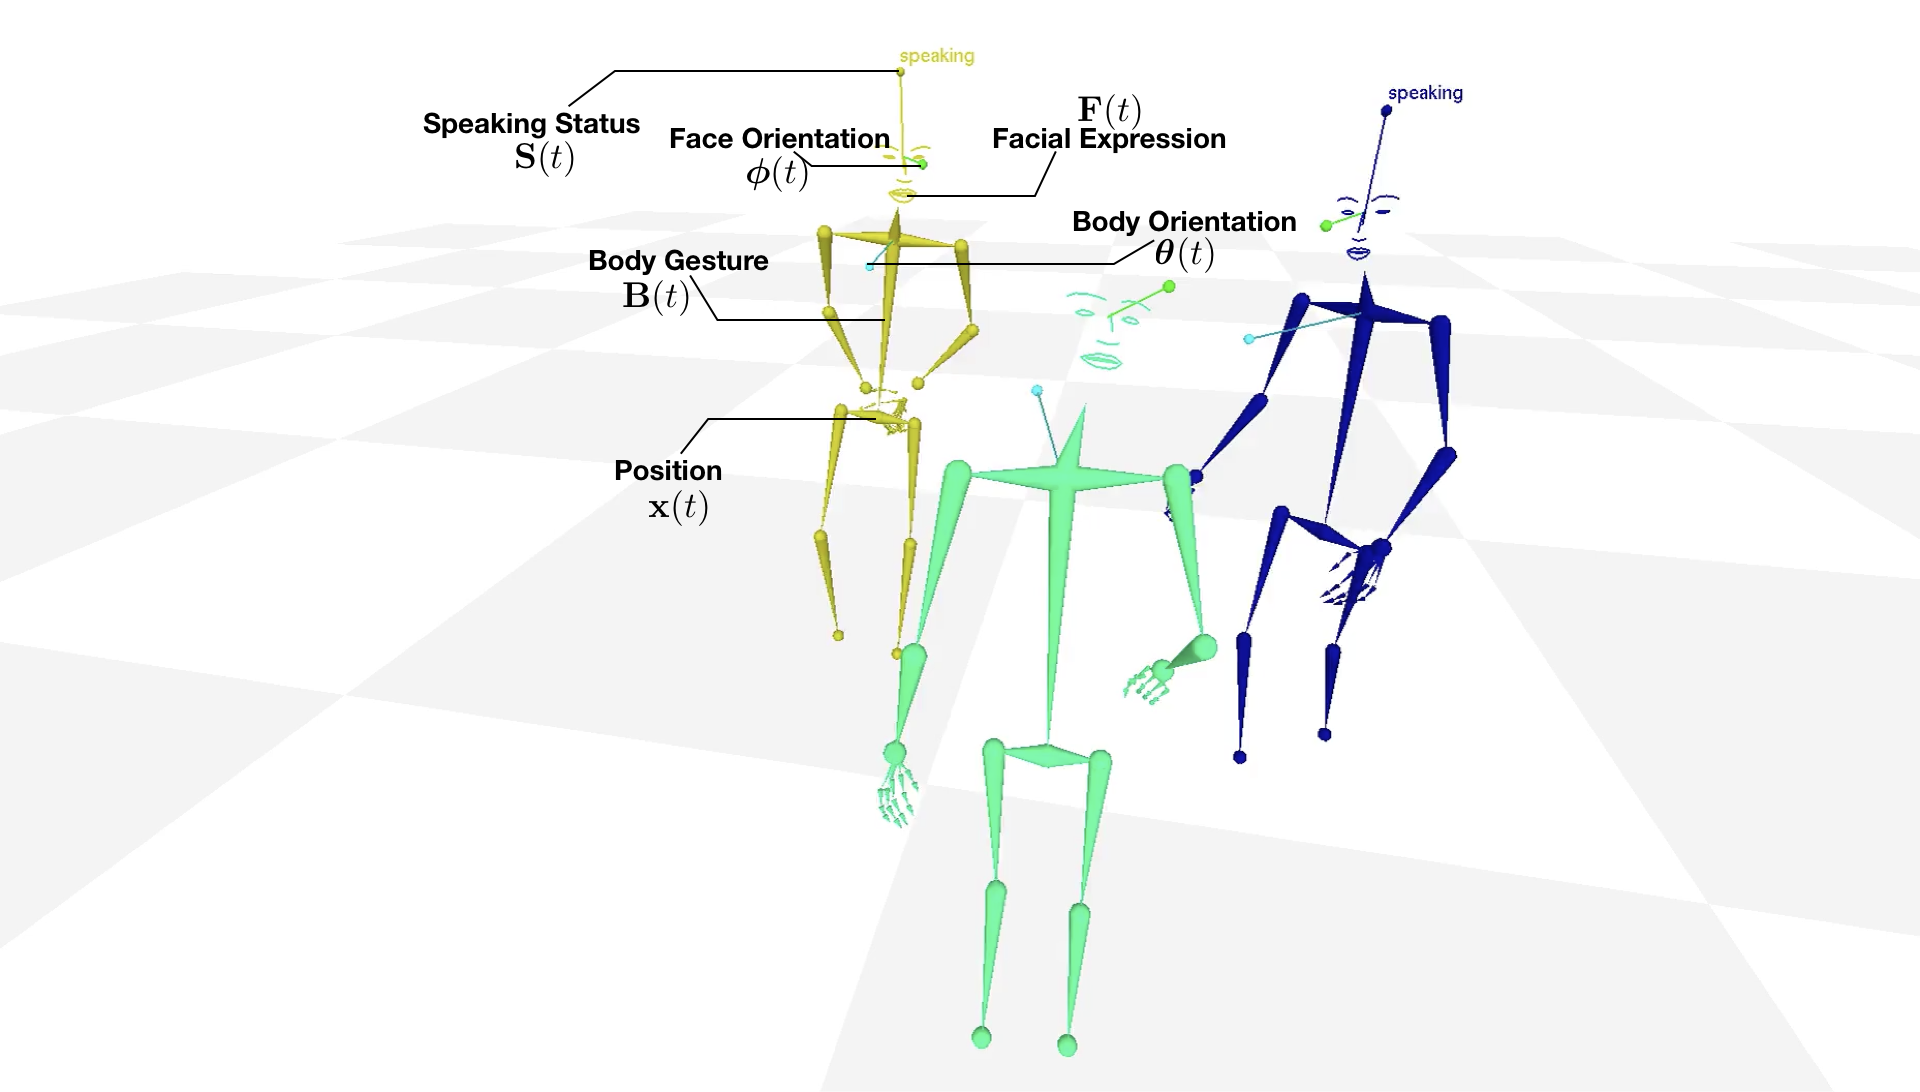
\includegraphics[trim=250 0 250 0,clip,height=0.3\linewidth]{ssp_fig/ssp_notation_input}
	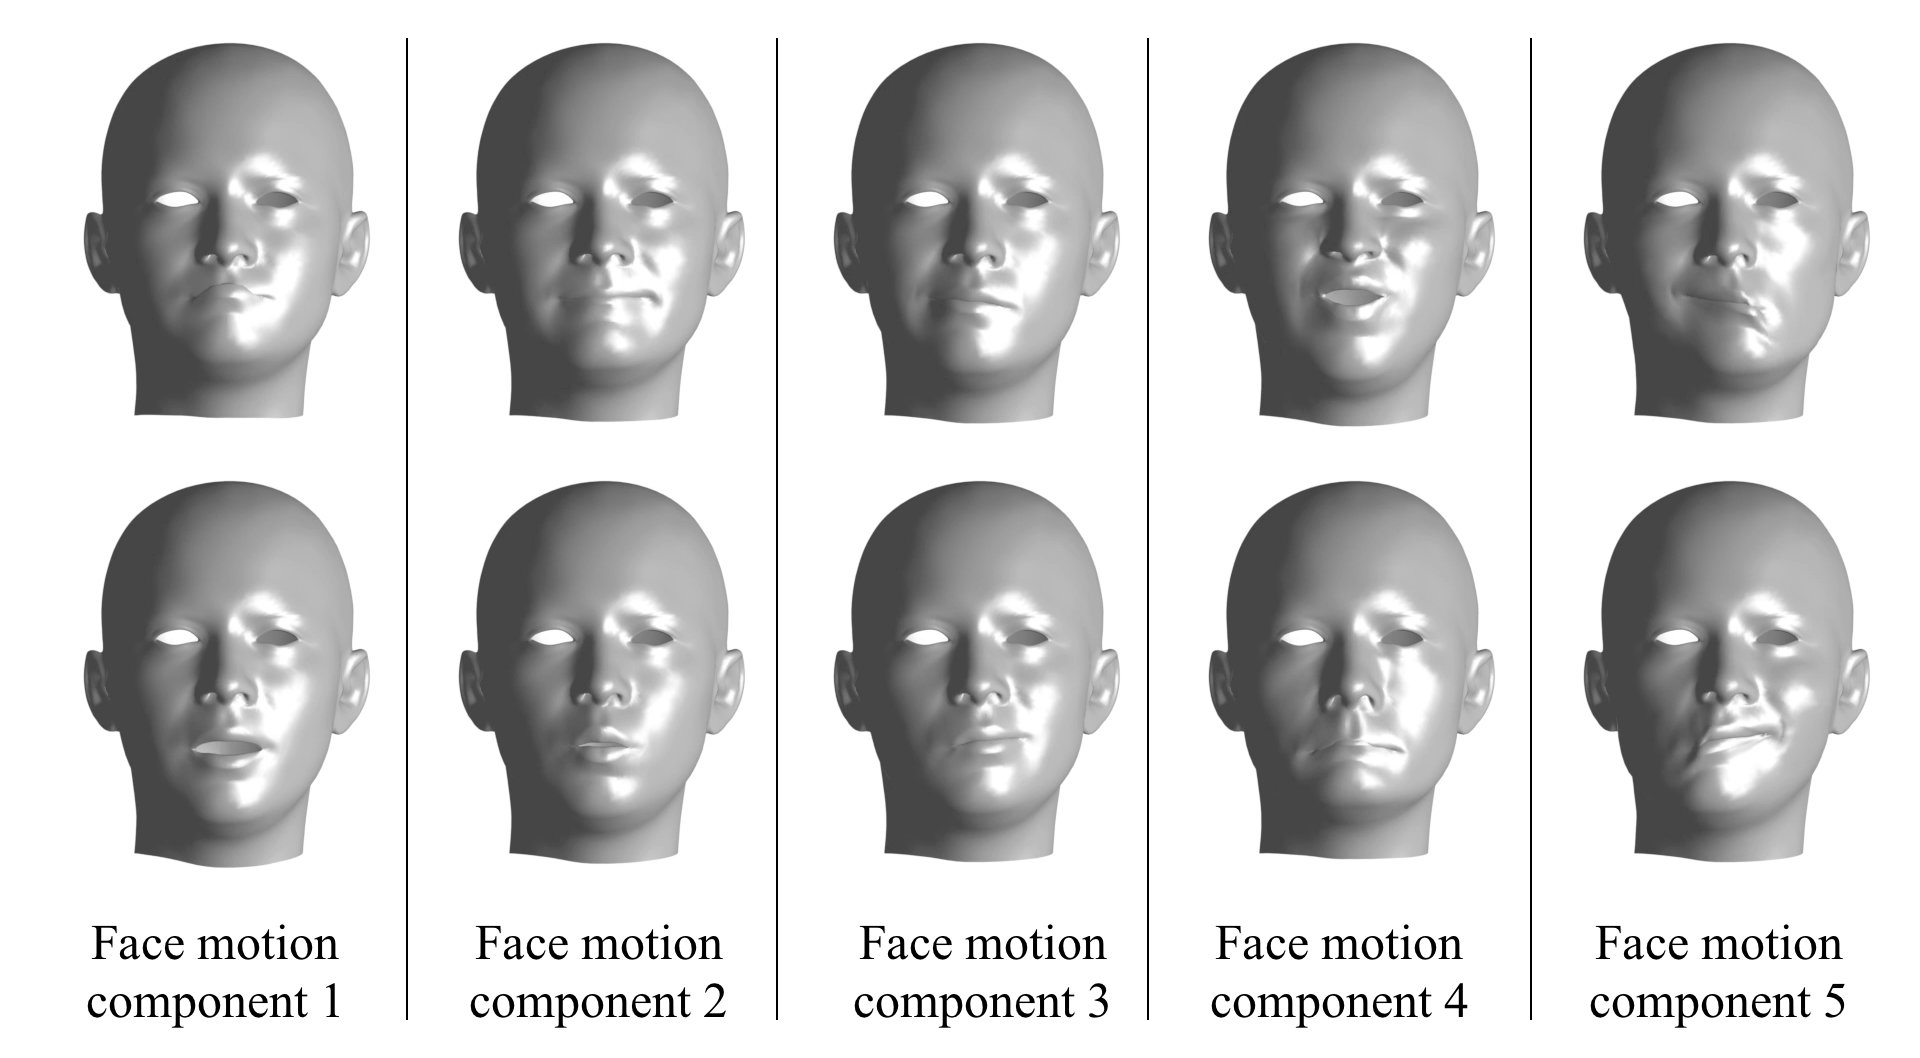
\includegraphics[trim=10 10 10 10,clip,height=0.3\linewidth]{ssp_fig/facemotion_comp}
	\caption{Social signal measurements used for social signal prediction. (Left) Reconstructed 3D social signals showing the body, face,  global position, face orientation, body orientation, and speaking status. (Right) The five face motion components (showing -0.3 on the top and 0.3 on the bottom) used in our social signal modeling.}
	\label{fig:notation_input}
\end{figure}


\subsection{Notation}
Our measurement method in the Panoptic Studio reconstructs 3D body motion $\mathbf{B}(t)$ and 3D face motion $\mathbf{F}(t)$ for each individual at each time $t$\footnote{We do not use the hand motion measurement due to the occasional failures in challenging hand motions (e.g., when both hands are close to each other), making it hard to train our model. We, however, believe this cue plays an important role in social interaction, which needs to be considered in future direction.}. We also denote the global position of the body as $\mathbf{X}(t)$. From these measurements, we additionally compute the body orientation $\boldsymbol{\theta}(t)$ and face orientation $\boldsymbol{\phi}(t)$ by finding the 3D normal direction of torso and face, respectively. We describe the details below, and the left of Figure \ref{fig:notation_input} shows an example visualization.

%Some figures to explain this
\paragraph{Body Motion:} We follow the body motion representation of the work of Holden et al.~\cite{holden2016deep}, representing a body gesture at a frame as a 73-dimensional vector, $\mathbf{B}(t) \in \mathbb{R}^{73}$. This representation is based on the skeletal structure of CMU Mocap dataset~\cite{gross2001cmu} with 21 joints (63 dimensions), along with the projection of the root joint (the center of the hip joints) on the floor plane (3 dimensions), the relative body locations and orientations represented by the velocity values of the root (3 dimensions), and footstep signals (4 dimensions). The orientations are computed only on the $x$-$z$ plane with respect to the $y$-axis, and the location and orientation represent the changes from the previous frame rather than the absolute values, following the previous work~\cite{jain2016structural, holden2016deep}. In particular, the first 63 dimensions of $\mathbf{B}(t)$ represents the body motion in the person-centric coordinate, where the root joint is at the origin and torso is facing the $z$ direction. We perform a retargeting process to convert our original 3D motion data from the Panoptic Studio, where the skeleton definition is the same as COCO dataset~\cite{coco-14} in the global coordinate, to this body motion representation with a fixed body scale. Thus, in our final motion representation, individual specific cues such as heights or lengths of limbs are removed and only motion cues are kept.

\paragraph{Face Motion:} For the face motion signal, we use the initial 5 dimensions of the facial expression parameters of Adam model (described in Chapter~\ref{chapter:totalcapture}), because we found the remaining dimensions have an almost negligible impact on our reconstruction quality. Note that the face expression parameters in our Adam model (originally from the work of \cite{cao2014facewarehouse}) are sorted by their influence by construction and the initial components have more impact in expressing facial motion. To this end, face motion at a time instance is represented by a 5-dimensional vector, $\mathbf{F}(t) \in \mathbb{R}^{5}$, as shown in the right of Figure \ref{fig:notation_input}. Here, we also do not include individual-specific information (the face shape parameters varying for individuals) and only motion cues are kept.
 
\paragraph{Position and Orientation:} For the global position $\mathbf{x}(t)$ of each individual, we use the coordinate of the root joint of the body, ignoring the values in $y$ axis, and thus $\mathbf{x}(t) \in \mathbb{R}^2$.
We use a 2D unit vector to represent body orientations $\boldsymbol\theta (t) \in \mathbb {R}^2$ and face orientation $\boldsymbol\phi (t) \in \mathbb{R}^2$, defined on the $x$-$z$ plane ignoring the values in $y$ axis. Note that we use unit vectors rather than angle representation, because the angle representation has a discontinuity issue when wrapping around $2\phi$ and $-2\phi$. In contrast to the relative location and orientation represented in the part of body motion $\mathbf{B}(t)$, these $\mathbf{x}(t)$, $\boldsymbol\theta (t)$, and $\boldsymbol\phi (t)$ represent the values in the global coordinate, which are used to model social formation. In summary, the status of an individual at a frame in social formation prediction is represented by a 6-dimensional vector, $[\mathbf{x}(t)^{\top}, \boldsymbol{\theta}(t)^{\top}, \boldsymbol{\phi}(t)^{\top} ]^{\top} \in \mathbb{R}^6$.

\paragraph{Speaking Status:} The voice data $\mathbf{V}(t)$ of each individual is also recorded by wireless microphones assigned to each individual. From the audio signal, we manually annotate a binary speaking label $\mathbf{S}(t) \in \{0,1\}$ describing whether the target subject is speaking (labelled as $1$) or not speaking (labelled as $0$) at time $t$.\\%In summary we measure the following signals for each individual:
%\begin{equation}
%[ \mathbf{x}, \boldsymbol{\theta}, \boldsymbol{\phi}, \mathbf{J}, \mathbf{F}, \mathbf{H}, \mathbf{V}, \mathbf{S} ].
%\label{equation:measurement}
%\end{equation}
\mbox{ }\\
By leveraging these various behavioral cues measured in the Haggling scenes, we model the dynamics of these signals in a triadic interaction. The objective of our direction is to regress the function defined in Equation~\ref{equation:F_ours}. To further constrain the problem we assume that the target person is the seller positioned on the left side of the buyer, and as input we use the social signals of the buyer ($\mathbf{X}^1$) and the other seller ($\mathbf{X}^2$). Based on our social signal measurements, the input and output of the function are represented as,
\begin{equation}
\begin{gathered}
\mathbf{Y} = [ \mathbf{x}^0, \boldsymbol{\theta}^0, \boldsymbol{\phi}^0, \mathbf{B}^0, \mathbf{F}^0, \mathbf{S}^0 ],\\
\mathbf{X}^1 = [ \mathbf{x}^1, \boldsymbol{\theta}^1, \boldsymbol{\phi}^1, \mathbf{B}^1, \mathbf{F}^1, \mathbf{S}^1 ],\\
\mathbf{X}^2 = [ \mathbf{x}^2, \boldsymbol{\theta}^2, \boldsymbol{\phi}^2, \mathbf{B}^2, \mathbf{F}^2, \mathbf{S}^2 ],
\end{gathered}
\end{equation}
where we use the superscript 0 to denote the social signals of the target subject (the output of social signal prediction).

% \begin{figure*}
% 	\centering
% 	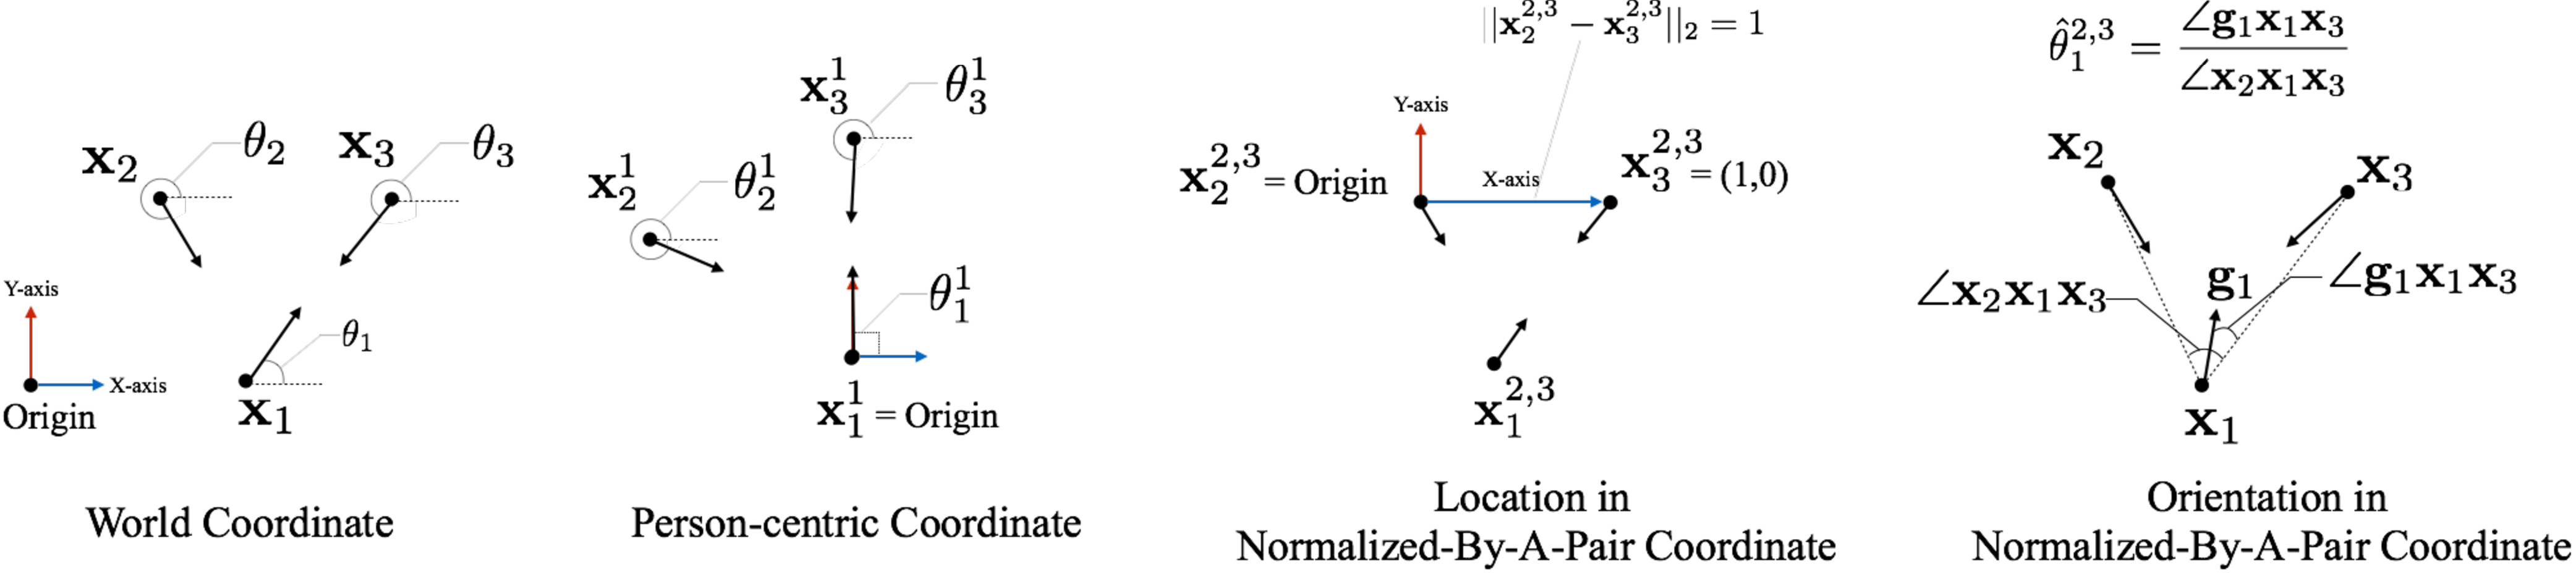
\includegraphics[width=\textwidth]{fig/ssp_notation3}
% 	\caption{Locations and orientations of an interacting group can be represented by different coordinate systems. (a) Locations and orientations in a world coordinate, (b) Locations and orientations in a person centric coordinate by person $\mathbf{P}_1$, (c) A location of $\mathbf{P}_1$  in a normalized coordinate by a pair of people $\mathbf{P}_2$ and $\mathbf{P}_3$, (d) An orientation of $\mathbf{P}_1$ in a normalized coordinate by a pair of people  $\mathbf{P}_2$ and $\mathbf{P}_3$. } 
% 	\label{fig:ssp_notation1}
% \end{figure*}

\subsection{Predicting Speaking}
\label{subsection:ssp_pred_speak}
%We predict whether the target subject is currently speaking or not, denoted by $\mathbf{S}^0$.  This is a binary classification task and we choose this task relatively easier to train. We first study the correlation between the speaking signal and the target person's own social signals, either body motion or facial motion, or both. We expect this correlation is stronger than the link between individuals. We train a similar model by using the conversational partner's social signals. In particular, we use the other seller's signals to predict the target seller's speaking status. More specifically, a function $\mathcal{F}_{B0\rightarrow S0}$ uses the target person's own body motion $\mathbf{B}^0(t_0:t)$ to predict the speaking signal:

We predict whether the target subject is currently speaking or not, denoted by $\mathbf{S}^0$.  This is a binary classification task and can be reliably trained by Cross Entropy loss function. We first study the correlation between the speaking signal of the target person, $\mathbf{S}^0$, and the person's own social signals, either body motion $\mathbf{B}^0$ or facial motion $\mathbf{F}^0$, or both. We expect this correlation is stronger than the link across individuals. Formally, a function $\mathcal{F}_{B0\rightarrow S0}$ uses the target person's own body motion $\mathbf{B}^0(t_0:t)$ to predict the speaking signal:
\begin{gather}	
\mathbf{S}^0(t_0:t) = \mathcal{F}_{B0\rightarrow S0} \left( \mathbf{B}^0(t_0:t) \right),
\label{eq:speaking_0}
\end{gather}
and similarly,
\begin{gather}	
\mathbf{S}^0(t_0:t) = \mathcal{F}_{F0\rightarrow S0} \left( \mathbf{F}^0(t_0:t) \right),\\
\mathbf{S}^0(t_0:t) = \mathcal{F}_{(F0, B0)\rightarrow S0} \left( \mathbf{F}^0(t_0:t) , \mathbf{B}^0(t_0:t)\right),
\label{eq:speaking_0_facebody}
\end{gather}
where $\mathcal{F}_{F0\rightarrow S0}$ uses the target person's own face motion, and $\mathcal{F}_{(F0, B0)\rightarrow S0}$ uses both. 

We compare the performance of these functions with the functions that takes the signals from a communication partner, the other seller:
\begin{gather}	
\mathbf{S}^0(t_0:t) = \mathcal{F}_{B2\rightarrow S0} \left( \mathbf{B}^2(t_0:t) \right),\\
\mathbf{S}^0(t_0:t) = \mathcal{F}_{F2\rightarrow S0} \left( \mathbf{F}^2(t_0:t) \right),\\
\mathbf{S}^0(t_0:t) = \mathcal{F}_{(F2, B2)\rightarrow S0} \left( \mathbf{F}^2(t_0:t), \mathbf{B}^2(t_0:t) \right),
\label{eq:speaking_1}
\end{gather}
where the functions use body cues, face cues, and both cues, respectively. 

This framework enables us to quantitatively investigate the link among social signals across individuals. For example, we may easily hypothesize that there exists a strong correlation between the signals from the same individual (e.g., speaking and facial motion of the target person), while the correlation between the signals across different individuals (e.g., speaking of the target person and body motion of another person) may be considered as weak. By comparing their performances, we verify there still exists strong links among these signals exchanged across subjects. 

%the social signals oindividual dynamics of the social signals is stronger than correlation between the speaking and the social signal body motion should be stronger than the speaking of the target and other people's body motions. But we still presume that there exists a clear correlation in building the function ~\ref{eq:speaking_1}; for example, if another person is talking we can guess the target person is not speaking due the ``turn-taking" implicitly followed during a social conversation. % This study is interesting because it demonstrates the existence of social correlation among social signals.

\paragraph{Implementation Details.}
Our neural network is composed of four 1-D convolutional layers, as shown in the top of the Figure~\ref{fig:ssp_imp_detail}. The first three layers output 128, 256, and 512 dimensional features respectively with ReLU activation functions, and the last layer has $1\times1$ convolutions with a sigmoid activation layer. Dropout~\cite{srivastava2014dropout} is also applied for the second and third layers with a retention probability of 0.25. Our model does not require a fixed window size for the input (since it is fully convolutional), but we separate input data into small clips with a fixed size (denoted by $f$) for the efficiency in training. During testing time, our models can be applied to the input of arbitrary length. We use $f=120$ (4 seconds) for the input window size for training, and we use an arbitrary length of input data for testing. The feature dimension of the input of our network is the concatenation of face motion and body motion (78 dimensions). If fewer cues are used (e.g., face only or body only), we mask out the unused channels as their average values computed in training set by keeping the same network structure. We use an adaptive gradient descent algorithm, AmsGrad algorithm~\cite{reddi2018convergence}, implemented in PyTorch~\cite{paszke2017automatic}, along with the $l^1$ regularization loss with the weight of 0.001. 

%The basic architecture follows the work of Holden et al.~\cite{holden2016deep} that demonstrates a compelling result for the mapping between a 2D trajectory and human motions. We modify the network architecture based on the input and output dimensions. 

%The network architecture is shown in the first row of Figure~\ref{fig:architectures}.
%\label{section:body2speak}
%The input of this network is the body motion of the other seller in the haggling sequence, which is a $f \times 73$ matrix, where $f$ is the number of frames of an input sequence. Here, we ignore the buyer's body motion because often little movement is observed from the buyers.  

\begin{figure}[t]
	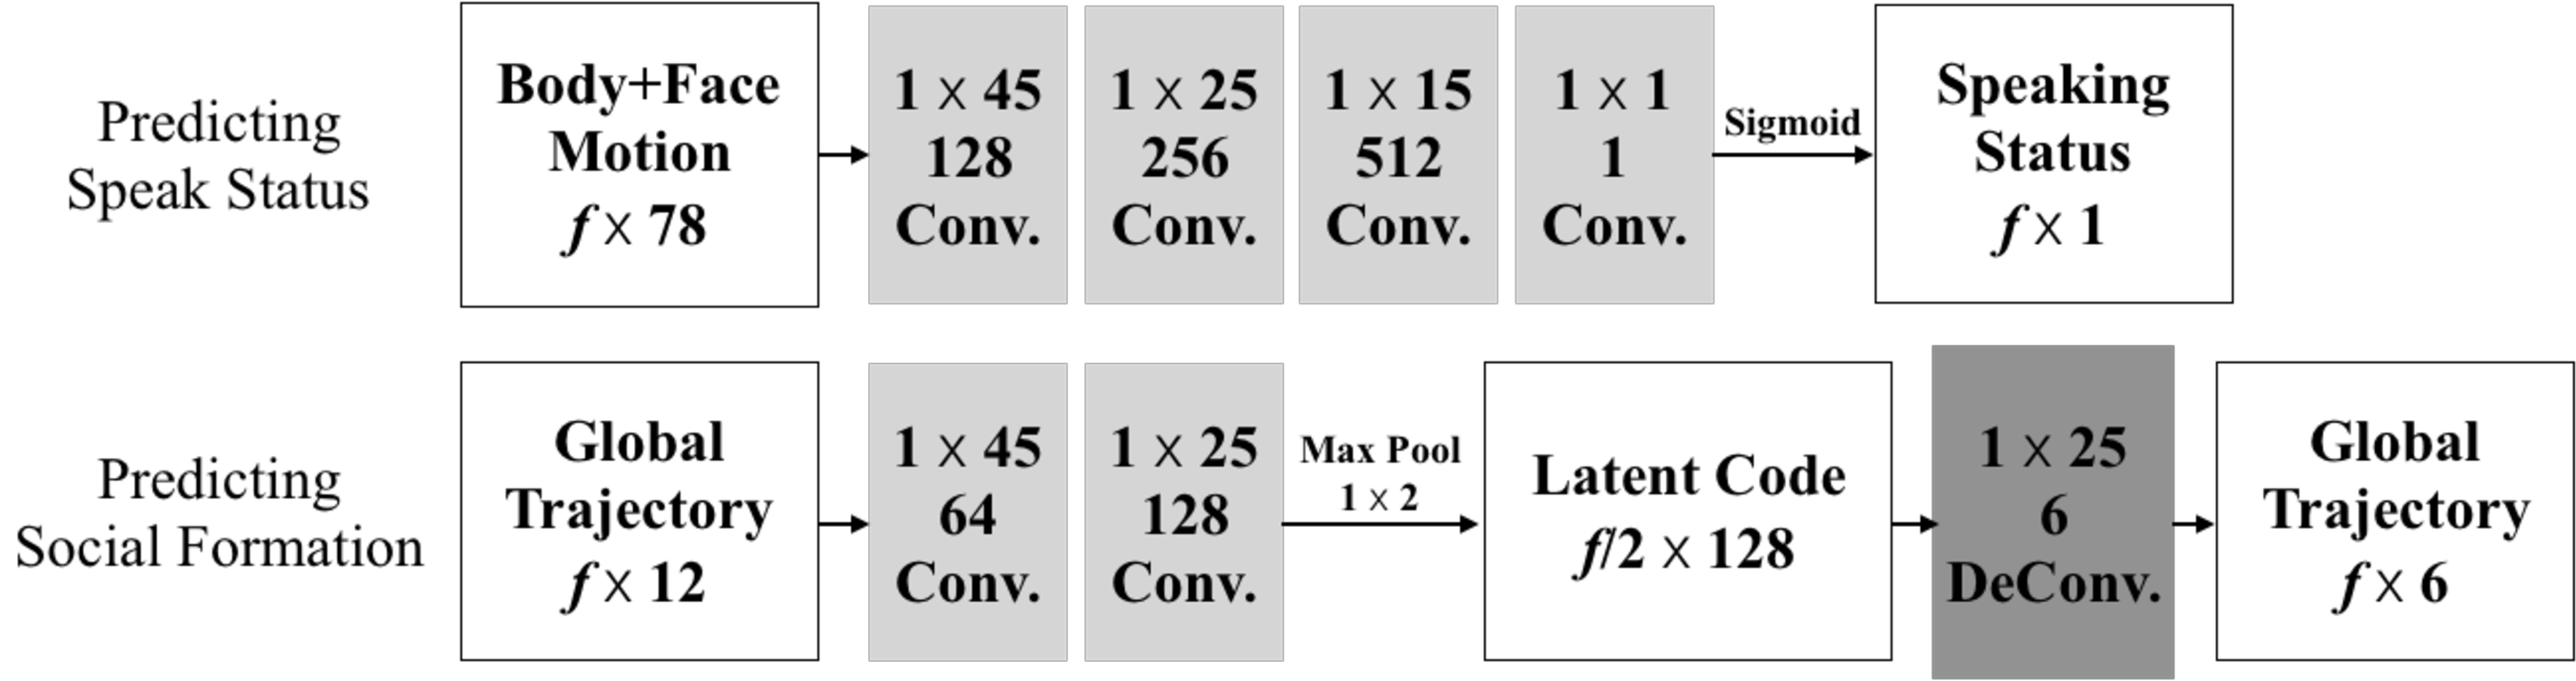
\includegraphics[width=\linewidth]{ssp_fig/ssp_imp_detail.pdf}
	\caption{Network Architectures. We use fully convolutional networks for both predicting speaking status and social formation problems. The models can be applied to the input of arbitrary length, but we use the input data of a fixed size $f=120$ for the efficiency in training.}
	\label{fig:ssp_imp_detail}
\end{figure}


\subsection{Predicting Social Formations}
We predict the location and orientations of the target person, denoted by $\mathbf{Y}_p = [{\mathbf{x}^0}^{\top}, {\boldsymbol{\theta}^{0}}^{\top}, {\boldsymbol{\phi}^{0}}^{\top} ]^{\top}$, given the same channels of cues from the communication partners. This problem is strongly related to Proxemics~\cite{Hall66} and F-formation~\cite{kendon90}, illustrating how humans use their space in social communications. Formally, 
\begin{gather}	
 \mathbf{Y}_p (t_0:t) = \mathcal{F}_p \left( \mathbf{X}_p^1(t_0:t), \mathbf{X}_p^2(t_0:t) \right),
 \label{eq:pred_formation}
\end{gather}
where $\mathbf{Y}_p$, $\mathbf{X}_p^1$, $\mathbf{X}_p^2$ contains global location and orientation signals $[{\mathbf{x}^i}^{\top}, {\boldsymbol{\theta}^{i}}^{\top}, {\boldsymbol{\phi}^{i}}^{\top} ]^{\top}$ (where $i=1,2$, or $3$) for the target subject and others.
Note that we only consider the positions and orientations on the ground plane (in 2D), ignoring the height of the subjects, and thus $\mathbf{Y}_p(t), \mathbf{X}_p^i(t) \in \mathbb{R}^6$. This prediction problem is intended to see whether the machine can learn how to build a social formation to interact with humans~\cite{vazquez2017towards}.

%Thus $\mathbf{x} \in \mathbb{R}^2 $ representing $x$ and $z$ coordinate of the subjects. We use a 2D unit vector to represent the orientations $\theta \in \mathbb {R}^2$ and face orientation $\phi \in \mathbb{R}^2$, because the angle representation has a discontinuity issue when wrapping around $2\phi$ and $-2\phi$. In summary, $\mathbf{X}^i(t)$ and $\mathbf{X}^i(t)$ are a $6 \times N$ dimensional matrix where $N = t- t_0$ is the size of the temporal window. T %We Social formation is one of the most noticeable social properties with strong correlation, allowing us to easily evaluate the performance.

\paragraph{Implementation Details.}
Our neural network has an autoencoder structure, where the encoder is composed of two 1-D convolutional layers followed by a max pooling layer with stride 2, and the decoder is composed of a single 1-D transposed convolution layer. The network is shown in the bottom of the Figure~\ref{fig:ssp_imp_detail}. The output feature dimensions are 64, 128, and 6 respectively. Dropout~\cite{srivastava2014dropout} is also applied in front of all layers with a retention probability of 0.25. Similar to the speaking status prediction, our model does not require a fixed window size for the input, but we separate input data into small clips with a fixed size ($f=120$, or 4 seconds) for the efficiency in training. The input is the concatenation of the cues of other two communication partners (12 dimensions) with a fixed order (buyer and then the right seller), and the output of our network is the position and orientations of the target individual, the left seller (6 dimensions). Similar to the previous prediction task, if fewer cues are used (e.g., position only), we mask out the unused channels as their average values computed in training set by keeping the same network structure. We use an adaptive gradient descent algorithm, AmsGrad algorithm~\cite{reddi2018convergence}, implemented in PyTorch~\cite{paszke2017automatic}, along with the $l^1$ regularization loss with the weight of 0.1.

%Our neural network is composed of four 1-D convolutional layers. The first three layers output 128, 256, and 512 dimensional features respectively with ReLU activation functions, and the last layer has $1\times1$ convolutions with a sigmoid activation layer. Dropout~\cite{srivastava2014dropout} is also applied for the second and third layers with a retention probability of 0.25. Our model does not require a fixed window size for the input, but we separate input data into small clips with a fixed size (denoted by $f$) for the efficiency in training. During testing time, our models can be applied to the input of arbitrary length. We use $f=120$, 4 seconds, for the input window size for training, and we use an arbitrary length of input data for testing. The feature dimension of the input of our network is the concatenation of face motion and body motion (78 dimensions). If fewer cues are used (e.g., face only or body only), we mask out the unused channels as their average values computed in training set by keeping the same network structure. We use an adaptive gradient descent algorithm, AmsGrad algorithm~\cite{reddi2018convergence}, implemented in PyTorch~\cite{paszke2017automatic}, and along with the $l^1$ regularization loss with the weight of 0.001.
%
%
%
%
%We use a 2D vector for the position and 2D unit vectors for the face orientation and body orientation, defined on the $xz$-plane. Thus the status of an individual at a frame in social formation prediction is represented by a 6-dimensional vector.
%
%
%The input of the social formation network is the concatenation of global position and orientation information of the communication partners, represented by a $f \times 12$ matrix.  We use a simple autoencoder structure, as shown in the second row of Figure~\ref{fig:architectures}.


%To implement this, we use a simple 1-D temporal convolutional neural network to model $\mathcal{F}_p$. The network is trained with a window of frames $N=120$ (corresponding to 4 seconds), but arbitrary length of input can be used in testing time since our network is fully convolutional. We use a simple encoder-decoder network. The encoder has  3 convolutional layers followed by dropout (0.25) and RELU, and 1D pooling layer (with stride 2). The decoder uses a single transposed convolution layer. We use L2 loss function with a L1 regularization term (with weight 0.1). We simply use the global position and orientations with standardization, rather than any local or relative coordinate.
